\chapter{\texttt{ilcsoft}}

\section{Projet \nnhAnalysis}

\section{Programme \processor}

\subsubsection{Données}
Initialement, on m'a mis à disposition des fichiers \SLCIO rangés par processus dans 66 dossiers (Figure~\ref{listeProcessus}).

\begin{figure}[h!]
	%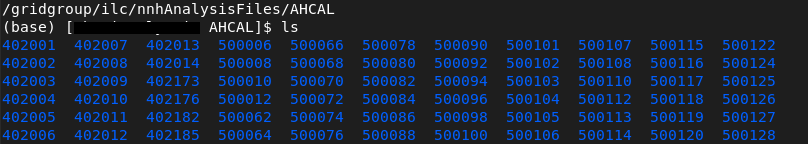
\includegraphics[width=\textwidth]{../img/listeProcessus.png} 
	\caption{Les noms des dossiers qui correspondent aux numéros de processus}
	\label{listeProcessus}
	
\end{figure}

\paragraph{Numéro des processus ???}

%\paragraph{Résultats mis à disposition ???}

\subsubsection{Méthodes}

On cherche à convertir ces fichiers \SLCIO en arbre \ROOT par processus.

\subsubsection{Résultats}

%\paragraph{Des fichiers \ROOT :}
Chaque dossier de fichier de donnée \SLCIO produira un fichier \ROOT en sortie, \cad que l'on obtiendra un arbre \ROOT par processus.


\subsubsection{Interprétation}

\section{Programme \analysis}

\subsubsection{Données}

On récupère les fichiers \ROOT du programme \processor précédent. 

$ hadd $ qui va créer le fichier DATA.root

\subsubsection{Méthodes}

\paragraph{\texttt{BDT}}

Entrainement

\paragraph{L'analyse}



\subsubsection{Résultats}

\paragraph{Vérification des résultats}
Comparaison entre les différents séries d'analyse, basée sur les même fichiers \ROOT, mais un autre entraînement de BDT.

\subsubsection{Interprétation}